% Created 2022-04-14 Thu 01:44
% Intended LaTeX compiler: pdflatex
\documentclass[12pt]{extarticle}
\usepackage[utf8]{inputenc}
\usepackage[T1]{fontenc}
\usepackage{graphicx}
\usepackage{longtable}
\usepackage{wrapfig}
\usepackage{rotating}
\usepackage[normalem]{ulem}
\usepackage{amsmath}
\usepackage{amssymb}
\usepackage{capt-of}
\usepackage{hyperref}
\usepackage{minted}
\usepackage[french]{babel}
\usepackage{tree-dvips}
\usepackage{titlesec}
\usepackage{fontspec}
\usepackage[top=2.54cm, bottom=2.54cm, left=1.91cm, right=1.91cm]{geometry}
\usepackage{graphicx}
\usepackage{setspace}
\usepackage{tikz}
\usepackage{hyperref}
\usepackage{xcolor}
\usepackage{float}
\usepackage{listings}
\usepackage{minted}
\usepackage[font=bf, skip=2pt]{caption}
\usepackage[most,listings]{tcolorbox}
\usepackage[style=apa] {biblatex}
\usepackage{xurl}
\usepackage{subfig}

\defaultfontfeatures{Mapping=tex-text,Scale=MatchLowercase}
\setmainfont{Open Sans}
\setmonofont{Consolas}
\floatstyle{plaintop}
\restylefloat{table}
% \titleformat{\paragraph}
% {\normalfont\normalsize\bfseries}{\theparagraph}{1em}{}
% \titlespacing*{\paragraph} {0pt}{3.25ex plus 1ex minus .2ex}{1.5ex
%   plus .2ex}

% \titlespacing{\section}{0pt}{\parskip}{-\parskip}

\graphicspath{{./img/}}

% \tcbset{colframe=white}

\hypersetup{
  colorlinks,
  linkcolor={red!50!black},
  citecolor={blue!50!black},
  urlcolor={blue!80!black}
}

\lstset{
  basicstyle=\ttfamily,
  backgroundcolor=\color{gray},
  showstringspaces=false,
  commentstyle=\color{red},
  keywordstyle=\color{blue}
}

\definecolor{monokaibg}{HTML}{272822}
\definecolor{borlandbg}{HTML}{eeeeee}
\definecolor{sectionbg}{HTML}{56b0c9}
\definecolor{titlepagebg}{HTML}{44899d}
% \definecolor{Text}{HTML}{FFFFFF}
% \AtBeginEnvironment{minted}{\color{Text}}

\newcommand{\csection}[1]{
  \begin{tcolorbox}[colback=sectionbg]
    \section{#1}
  \end{tcolorbox}
  \noindent
}


\newcommand{\titre}[1]{
\vfill
\begin{spacing}{1.2}
\huge\textsc{#1}
\end{spacing}
\vfill
}
\newcommand{\cours}[1]{{\Large\textsc{#1}}}
\newcommand{\groupe}[1]{{\Large #1}}

\newenvironment{ctitlepage}
{\cleardoublepage\begin{titlepage}\thispagestyle{empty}\begin{center}
      
\includegraphics[scale=1]{polylogo.png}
      \vfill}
    {\end{center}\end{titlepage}}

\onehalfspacing
\addbibresource{template.bib}
\let\cite\parencite
\date{}
\title{Template}
\begin{document}

\begin{ctitlepage}

\cours{INF8215}

\groupe{Groupe 01}

\titre{\textbf{TP3} \\
Classifications multiclasses:\\
légumes secs}

\vspace{.1in}

\textbf{Par} \\
Brando, Tovar \textbf{1932052} \\
Vega, Estefan \textbf{1934346} \\
Équipe: \textbf{BrandiniStifini} \\

\vspace{.5in}

Le \today

\end{ctitlepage}

\newpage
\tableofcontents
\newpage


\section{Contexte}
\label{sec:org812d05c}
Dans ce travail pratique, il nous était demander de classifier des légumes secs dans leur catégorie respectives. Il y en avait 7 en tout; Sira, Horoz, Dermason, Barbunya, Cali, Bombay, Seker et nous devions déterminer la catégorie à l'aide de 16 \emph{features}. Nous avions donc à résoudre un problème de classification multiclasses. Nous avons décider d'utiliser la librairie \emph{scikit-learn} et le modèle que nous avons utilisé se base sur les machines à vecteurs de support (\emph{SVC OneVsOneClassifier}). Nous avons aussi exploré d'autres modèle telles que celui basée sur la descente de gradient stochastique (\emph{SGDClassifier}) et celle basée sur les forêts aléatoires (\emph{RandomForestClassifier})

\section{Prétraitement}
\label{sec:org60e422f}
Avant de commencé à résoudre le problème, il est utile de se familiariser avec les données. Nos données étaient constitué de 16 \emph{features}. Il y avait 6000 données de test. Nous avons commencé par voir s'il manquait des valeurs dans certaines de no données test ce qui n'était pas le cas. Nous avons ensuite regardé si nos donées étaient balancées.
\vspace{5mm}

\begin{minipage}{.45\textwidth}
\begin{center}
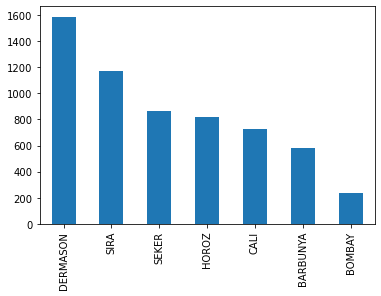
\includegraphics[width=\linewidth]{./.ob-jupyter/0e36c24725fa023c6e39f07bc9df640645c86811.png}
\end{center}
\vspace*{-5mm}
\captionof{figure}{Diagramme à bandes des catégories}
\label{fig:figure1}
\end{minipage}
\begin{minipage}{.55\textwidth}
\begin{center}
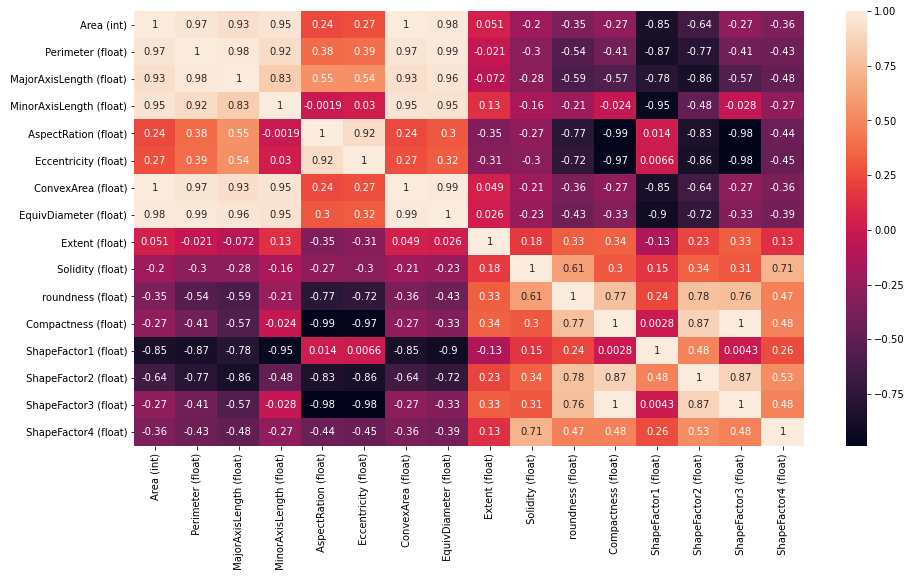
\includegraphics[width=\linewidth]{./.ob-jupyter/da88383af5d1618a3cb0bf8008eb6ce0c4c86bce.png}
\end{center}
\vspace*{-5mm}
\captionof{figure}{Matrice de corrélation}
\label{fig:figure2}
\end{minipage}

\vspace{5mm}

Il a été intéressant de voir qu'il y a présence de débalancement et que certains attributs étaient très corrélés entre eux soit > 0.9 ou < -0.9. Nous avons essayer de retirer les attributs corrélées, mais il n'y a pas vraiment eu de gain et nous avons donc décider de garder tous les attributs.

Une fois les analyse de données terminées, nous avons dû faire quelques changement dans les données afin de pouvoir utiliser notre modèle. Nous avons en premier lieu, dû transformer les valeurs de X\_train (attributs) en float. Nous avons ensuite retirer les valeurs de \emph{ID} dans X\_train et y\_train. Nous pouvions ainsi entrainer notre modèle. Étant données les mauvais résultats initiaux, nous avons dû faire appel à la normalisation. Nous sommes donc passées d'une précision de 0.268 à une de 0.933 sur le classificateur SVM.

\section{Méthodologie}
\label{sec:org94ef7a2}
\section{Résultats}
\label{sec:org6d04546}
\section{Discussion}
\label{sec:org93a931b}

\section{stuff}
\label{sec:orgbd765b7}
\begin{minipage}{.5\textwidth}
\begin{center}
\begin{tabular}{|r|rrr|rr|}
\hline
N & N\textsuperscript{2} & N\textsuperscript{3} & N\textsuperscript{4} & sqrt(n) & sqrt[4](N)\\
\hline
1 & 1 & 1 & 1 & 1 & 1\\
2 & 4 & 8 & 16 & 1.4142 & 1.1892\\
3 & 9 & 27 & 81 & 1.7321 & 1.3161\\
\hline
\end{tabular}
\end{center}
\vspace*{-5mm}
\captionof{table}{A table}
\label{tbl:table1}
\end{minipage}
\begin{minipage}{.5\textwidth}
\begin{center}
\begin{tabular}{|r|rrr|rr|}
\hline
N & N\textsuperscript{2} & N\textsuperscript{3} & N\textsuperscript{4} & sqrt(n) & sqrt[4](N)\\
\hline
1 & 1 & 1 & 1 & 1 & 1\\
2 & 4 & 8 & 16 & 1.4142 & 1.1892\\
3 & 9 & 27 & 81 & 1.7321 & 1.3161\\
\hline
\end{tabular}
\end{center}
\vspace*{-5mm}
\captionof{table}{Another table}
\label{tbl:table2}
\end{minipage}

\begin{table}[htbp]
\caption{\label{tbl:table3}Regular table}
\centering
\begin{tabular}{|r|rrr|rr|}
\hline
N & N\textsuperscript{2} & N\textsuperscript{3} & N\textsuperscript{4} & sqrt(n) & sqrt[4](N)\\
\hline
1 & 1 & 1 & 1 & 1 & 1\\
2 & 4 & 8 & 16 & 1.4142 & 1.1892\\
3 & 9 & 27 & 81 & 1.7321 & 1.3161\\
\hline
\end{tabular}
\end{table}

\begin{listing}[htbp]
\begin{minted}[breaklines=true,breakanywhere=true,linenos=true,gobble=-8,xleftmargin=20pt,bgcolor=borlandbg]{shell}
ls -l
\end{minted}
\caption{Source code}
\end{listing}

\begin{center}
\begin{tabular}{lrllrlrrl}
total & 256 &  &  &  &  &  &  & \\
-rw-rw-r-- & 1 & bndo & bndo & 1406 & Apr & 13 & 21:12 & config.tex\\
drwxrwxr-x & 2 & bndo & bndo & 4096 & Apr & 13 & 23:18 & img\\
drwxrwxr-x & 2 & bndo & bndo & 4096 & Apr & 13 & 23:34 & \_minted-report\\
-rw-rw-r-- & 1 & bndo & bndo & 459 & Apr & 13 & 21:12 & packages.tex\\
-rw-rw-r-- & 1 & bndo & bndo & 1378 & Apr & 13 & 21:12 & README.org\\
-rw-rw-r-- & 1 & bndo & bndo & 2978 & Apr & 14 & 01:24 & report.bbl\\
-rw-rw-r-- & 1 & bndo & bndo & 7162 & Apr & 14 & 01:44 & report.org\\
-rw-rw-r-- & 1 & bndo & bndo & 214812 & Apr & 14 & 01:24 & report.pdf\\
-rw-rw-r-- & 1 & bndo & bndo & 5780 & Apr & 14 & 01:24 & report.tex\\
-rw-rw-r-- & 1 & bndo & bndo & 738 & Apr & 13 & 21:12 & template.bib\\
\end{tabular}
\end{center}


\section{Section 2}
\label{sec:org2a13753}
\newpage


selon une etude \cite{2021}

\newpage

\phantomsection
\addcontentsline{toc}{section}{Références}

\printbibliography
\end{document}
